\chapter{Problemløsning}
\label{cha:problemlosning}
\frnote{mangler intro}

Der er blevet udarbejdet en problemformulering og en kravspecifikation. Ud fra dette skal der laves en løsning. Ifølge studieordningen skal der udarbejdes et større program af høj kvalitet. Det er også et krav at programmet skal skrives i C\#. I dette kapitel vil der være en beskrivelse af denne løsning. Der vil blive beskrevet hvordan løsningen blev lavet. Der vil blive gjort rede for det overordnede design af løsningen. C\# er oprindeligt lavet af Microsoft og bruges primært på Microsofts Windows styresystem. Derfor laves løsningen et Windows program i Microsoft Visual Studio. Til programmet er også lavet en simpel brugergrænseflade. Et Windows program passer godt til Vestre Baadelaug, da de allerede anvender Windows-baserede systemer til administrationen.

\kanote{ovenstående skal tages op til overvejelse}

%!TEX root = ../../Master.tex
\section{Usecases}

\subsection{Usecases:}

\begin{itemize}
  \item Gæst vil finde en plads:
  \begin{itemize}
    \item 1) Ny gæst melder til systemet, hvor lang tid han vil ligge til.
    \item 2) Systemet returnerer en liste over pladser som vil passe hans behov.
    \item 3) Gæsten vælger en plads som passer til hans båd.
    \item 4) Systemet melder at pladsen er nu reserveret (rød lampe).
    \item 5) Gæsten betaler for pladsen.
    \item 6) Systemet melder til havnefogeden at der er nye ankomne.

    \item Alternativ: De tre første 2 skridt er ikke nødvendige.
  \end{itemize}

  \item Medlem forlader sin plads:
  \begin{itemize}
    \item 1) Medlemmer melder til systemet tidspunkt for afrejse og hjemkomst.
    \item 2) Systemet venter til efter afrejse tidspunktet.
    \item 3) Når pladsen tømmes, da melder systemet at pladsen er fri (grøn lampe).
  \end{itemize}

  \item Medlem vender tilbage til sin plads:
  \begin{itemize}
    \item 1) Systemet registrerer når medlemmet ligger til, og melder at plads er optaget (rød lampe).
  \end{itemize}

  \item Havnefogeden melder plads optaget:
  \begin{itemize}
    \item 1) Medlem ringer til havnefogeden og fortæller om tidlig hjemkomst.
    \item 2) Havnefogeden indtaster (ny) dato i systemet.
    \item 3) Systemet returnere enten a eller b
    \item a) Dato er accepteret
    \item 1b) En gæst har lejet pladsen for en længere periode.
    \item 2b) Systemet foreslår en ny plads til gæsten.
    \item 3b) Havnefogeden snakker med gæsten.
  \end{itemize}

  \item Automatisk arrangementsforslag:
  \begin{itemize}
    \item 1) Antallet af medlemmer i havnen overstiger et bestemt niveau.
    \item 2) Systemet melder at det ville være en god dag for et arrangement.
    \item 3) Et medlem af klubben ser denne melding, og foreslår et arrangement.
  \end{itemize}

  \item Automatisk medlemstjek
  \begin{itemize}
    \item 1) Systemet registrerer uoverensstemmelse med angivet rejseplan.
    \item 2) Systemet notificerer havnefogeden omkring overensstemmelsen.
  \end{itemize}
  

\end{itemize}



\chapter{Relevant Teori for Design og Implementation}

\kanote{intro tekst}

\section{Internet of Things} % (fold)
\label{sec:internet_of_things}
Som en del af løsningen skal der indgå en sensorer, der kan detektere både i havnen. For at finde ud af mere, om hvad der er muligt, er konceptet \enquote{Internet of Things}, herefter IoT, blevet undersøgt. IoT er et paradigme, hvor alle fysiske genstande skal være unikt identificerbare, således at computere nemmere kan administrere disse genstande. Derudover handler IoT om at forbinde disse genstande i et netværk \cite{kopetz2011real}. En mere beskrivende definition af IoT er derfor \enquote{a world-wide network of interconnected objects uniquely addressable, based on standard communication protocols} \cite{iot_survey_2010}.

\subsection{Konceptet}
\label{sub:iot_koncept}
IoT er ofte beskrevet ud fra forskellige visioner for paradigmet. I \cite{iot_survey_2010}  beskrives tre visioner; \enquote{Things oriented}, \enquote{Internet oriented} og \enquote{Semantic oriented}. Disse visioner er opstået ud fra de forskellige interessenter i IoT. Disse interessenter angriber IoT fra forskellige vinkler og er derfor kommet fra til forskellige definitioner af IoT. Se \cref{fig:iot_visions}.

Den første definition af IoT, \enquote{Things oriented}, stammer fra Auto-ID labs, et verdensomspændende netværk af forskere indenfor Radio Frequency IDentification (RFID) og anden sensor teknologi. Målet med IoT er i denne definition at forbedre synligheden og muligheden for at spore genstande. For at opnå dette er Electronic Product Code (EPC) standarden blevet udviklet. Denne standard har til formål at sprede brugen af RFID samt andre teknologier \cite{iot_survey_2010}.

Den anden vision for IoT, \enquote{Internet oriented}, bygger videre på den første definition. Denne vision består i, at alle objekter selv kan forbinde sig til hinanden og computere. Konsortiummet CASAGRAS har fokus på at skabe \enquote{a world where things can automatically communicate to computers and each other, providing services to the benefit of the human kind} \cite{iot_survey_2010}.

Den sidste vision der beskrives her, \enquote{Semantic oriented}, omhandler hvordan de data, der genereres i \enquote{Things oriented} delen af IoT, organiseres. Visionen behandler strukturering af store mængder data, med hensigten at der opnås en forbedret overskuelighed og menneskelig forståelse, af disse ellers ofte overvældende mængder data \cite{iot_semantics_2012}.


\begin{figure}
  \centering
  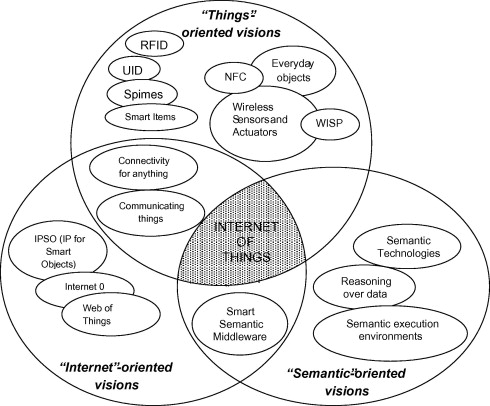
\includegraphics[width=\textwidth]{iot_visions}
  \caption{Internet of Things paradigmet ud fra tre visioner. Fra \cite{iot_survey_2010}.}
  \label{fig:iot_visions}
\end{figure}

\subsection{RFID}
RFID står for Radio Frequency IDentification, og som navnet antyder kan teknologien identificere objekter ved hjælp af radio frekvenser. Et RFID-tag, er en lille chip der indeholder en antenne, og en lille mængde data. Et objekt med et RFID-tag er nu \enquote{tagget}, og data om objektet kan læses ved hjælp af en RFID læser. Man kategoriserer typisk RFID-tags i passive og aktive. Et aktivt RFID-tag kræver strøm for at blive læst, og er derfor ofte tilsluttet et batteri. Et passivt RFID-tag kræver ingen strøm fra et batteri, men får derimod strømmen fra RFID-læseren \cite{want2006rfid}.

\subsection{Anvendelse af Internet of Things på Vestre Bådehavn}
\label{sub:iot_vestre_baadehavn}

Som beskrevet i \cref{sub:iot_koncept}, er der mange muligheder for hvilke sensorer der kan benyttes til at identificere objekter. Dette afsnit vil se på RFID og ultralyds sensorer, samt kameraer med billedgenkendelses software, som mulige sensorer, der kan benyttes på en havn som Vestre Bådehavn.

Lad os antage at alle både er blevet tagget med passive RFID-tags, sådan at de hver har en unik identifikation. Passive RFID-tags vægles da de er billige, og kan sidde på både uden nogen direkte afhængighed af elektricitet. Derudover kan hver vandlejeplads registrere, ved hjælp af en sensor, hvorvidt vandlejepladsen er optaget. Hvis der ligger en båd, kan en anden sensor også se hvem der ejer båden.

Sensoren som registrerer hvorvidt der ligger en båd på en vandlejeplads, kunne være en ultralyds sensor. Denne kan ved hjælp af lydbølger detektere tilstedeværelse af et objekt. Den kan dog ikke med stor præcision identificere objektet. En anden løsning er et kamera der ved hjælp af billed genkendelse kan identificere båden.

En computer forbundet til disse to typer sensorer, kan nu effektivt administrere en kæmpe havn med mange vandlejepladser. Når en ny båd lægger til på en vandlejeplads, vil computeren med det samme vide dette. Computeren kan derudover også kategorisere båden som en medlemsbåd eller som en gæstebåd. Da computeren nu har registreret at vandlejepladsen er optaget, skal den vende et skilt eller tænde for en diode, eller på anden måde ændres pladsens status til optaget.


\subsection{Opsummering}

I dette projekt arbejdes der udelukkende på en software løsning, og ikke på implementering af hardware. Derfor vil sensorerne som skal registrere bådene i havnen, blot blive simuleret, da deres tekniske opbygning ikke er direkte relevant for implementeringen af software løsningen. 

De simulerede sensorer kan opfatte tre tilstande. Enten kan den registrere at der ligger en ukendt båd, en kendt båd, eller ingen båd. Den ukendte båd vil være en gæst, og den kendte båd et medlem. Når en sensor opfanger et skift fra én tilstand til en anden, vil den sende et signal til softwareløsningen med info om den nye tilstand.

Det vurderes, på baggrund at den stigende interesse for \enquote{Internet of Things}, at denne slags sensorer er en del af en realistisk fremtidshorisont. Dette er en væsentlig forudsætning for den følgende løsningsmodels udgangspunkt.

\section{Teori om Klasser i C\#}
\label{sec:klasse_teori}

C\# er et objektorienteret programmeringssprog. I objektorienterede programmeringssprog er det let at dele programmer op, og på den måde lave mere velorganiserede programmer, der nemmere vedligeholdes. En af grundsøjlerne bag det objektorienterede paradigme, er objekter. For at lave et objekt skal man definere en klasse, som er skabelonen for objektet. 

Klasser er ofte en abstraktion eller en modellering af et koncept eller gestande fra den virkelige verden. Da det objektorienterede programmeringsparadigme ønskes anvendt, skal en model konstrueres, der kan anvendes i forbindelse med løsningen af problemformuleringen. I denne løsning ønskes der en modellering af de koncepter og genstande, der findes på en havn, og dette er derfor blevet undersøgt. For hvert relevant koncept og genstand, er der indgået overvejelser omkring den optimale måde at modellere dem i klasser.

I afsnit \cref{sec:klasse_design} beskrives hvilke valg der er taget i forbindelse med modelleringen af forskellige koncepter og genstande i løsningen.

\subsubsection{Teori om Klassehierarki og Klassediagrammer}
\label{sub:uml_teori}

\frnote{læs dette afsnit}

For at bedre kunne opnå en optimal modellering sættes klasser ind i et klassehierarki for at øge overskueligheden. Et klassehierarki er en organisering af et sæt af klasser og deres indbyrdes relationer.
\frnote{noget om subklasser}

Et klassediagram beskriver opbygningen af et system ved at vise systemets klasser, deres attributter, metoder, og relationerne mellem objekter \cite{martin2006agile}. Et klassediagram er en af de vigtigste byggesten i objektorienteret modellering. Det kan bruges både til generel konceptuel modellering og til detaljeret modellering, der kan omsættes til kildekode. 

I et klassediagram er klasser repræsenteret med bokse. Boksen indeholder tre dele. Den første del indeholder navnet på klassen, Og hvilken type klasse det er. I C\# kunne det for eksempel være en normal klasse eller et interface. Den anden del indeholder klassens attributter. Den sidste del indeholder operationer som klassen kan foretage.

Flere klasser representerer med bokse kan samles i et klasse diagram. I et klassediagram kan man ved hjelp af pile vise relationer mellem klassen.

For at give et overblik over klassehierarkiet i løsningen, er der lavet et klassediagram efter UML standarden i afsnit \cref{sec:klasse_design}.

\subsection{MVC}

\enquote{Model-View-Controller}, herefter kaldt MVC, er et designmønster, der bruges til at strukturere software med en brugergrænseflade \cite{mvcLecture}. Mønsteret opdeler en given software applikation i tre sammenhængende dele. Det centrale komponent, \enquote{Model}, som indeholder data og modellerer problemområdet. Et ydre komponent, \enquote{View}, der afvikler den visuelle repræsentation af information til brugeren. Den tredje del, \enquote{Controlleren}, som implementerer systemets funktionaliteter. Fordelen ved MVC er at programmet struktureres på en måde, så programmets enkelte dele har en lav kobling. En lav kobling gør det nemmere at udskifte dele af et program, og derved bliver programmet nemmere at vedligeholde. For eksempel kan hele det grafiske framework udskiftes, ved blot at skifte det ydre \enquote{View} komponent ud. \Cref{fig:mvc} viser den tydelige strukturelle forskel på \enquote{Model}, \enquote{View} og \enquote{Controller} komponenterne.

\begin{figure}
  \centering
  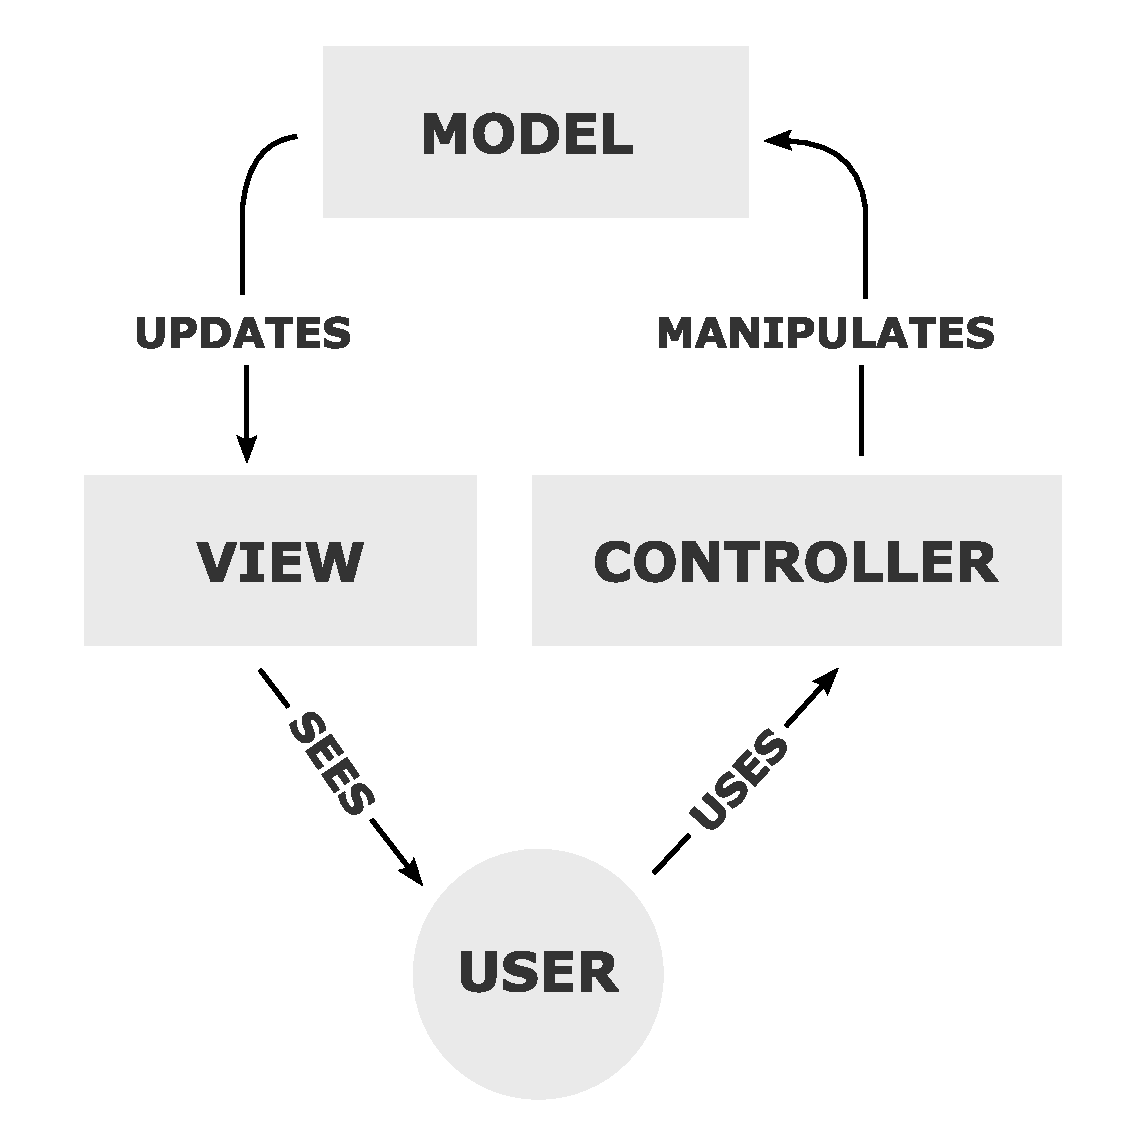
\includegraphics[width=0.75\textwidth]{mvc.pdf}
  \caption{Grundidéen omkring MVC. Fra \url{http://commons.wikimedia.org/wiki/File:MVC-Process.svg} } \label{fig:mvc}
\end{figure}



\section{Systematisk Test af Program}
\label{sec:systematisk_test_af_program}

\subsection{Test Driven Development}
\label{sub:test_driven_development}

For at sikre at programmet er let at teste, er kernefunktionerne i programmet udviklet jævnfør softwareudviklingsprocessen \enquote{Test Driven Development}. I Test Driven Development (TDD) skrives unit tests af en metode, før selve implementeringen af funktionen. Denne udviklingsprocess sikrer, at nye funktionaliteter ikke ødelægger de forud eksisterende \cite{martin2006agile}. Programmøren tvinges også til at tænke på, hvordan metoden bruges ved kald. Det sikres hermed, at metoden er overskueligt konstrueret, således at den kan kaldes uden unødigt besvær. Et andet aspekt af TDD, er at testkoden tjener som dokumentation af den testede metodes funktionalitet. Tilgengæld riskeres et øget tidsforbrug, der dog muligvis kan fraskrives fejlfinding.

\subsection{Unit Testing i Microsoft Visual Studio}
\label{sub:unit_testing_i_microsoft_visual_studio}

Microsofts unit test framework for managed code er anvendt til unit testing. Frameworket kan teste \enquote{managed code}, som C\# falder ind under. Når tests er skrevet, kan Test Explorer i Visual Studio køre testene. Når testene er færdige, vil resultaterne blive præsenteret som failed tests, passed tests, not run tests og skipped tests \cite{msdn_unittest}.

Før der skrives unit tests, skal der oprettes et unit test projekt. Herefter kan der tilføjes klasser annoteret med \enquote{[TestClass]}. Inde i disse klasser, tilføjer man de metoder, annoteret med \enquote{[TestMethod]}, som skal køres. Et eksempel på en test metode, kan se i \cref{lst:test_notfound}.
Alle tests til systemet kan findes på CD'en der afleveres som bilag.

\begin{lstlisting}[label=lst:test_notfound, caption={Eksempel på testfunktion}]
  [TestMethod]
  public void ShouldThrowWhenNotFound()
  {
      var space = new WaterSpace(404404, 4.3, 5.4);
      try
      {
          var test = BoatDetector.BoatAt(space);
      }
      catch (KeyNotFoundException _)
      {
          return;
      }
      Assert.Fail("No exception was thrown.");
  }
\end{lstlisting}



\begin{figure}
  \centering
  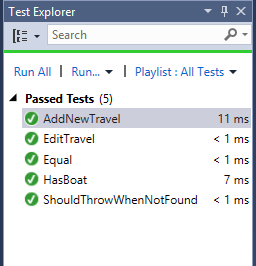
\includegraphics{test_explorer.png}
  \caption{Resultat af tests i Test Explorer i Visual Studio 2013}
  \label{fig:test_explorer}
\end{figure}

\subsection{Database}
\label{sub:database}



\section{Database} 
\label{sec:database}

En database er en organisering af en mængde data, ved brug af tabeller. En database bruges til at håndtere opgaver såsom, at gemme, hente eller søge i ofte store mængder lagrede data. En normal fil kan ikke skrives til, fra flere processer på samme tid, hvor en database derimod kan håndtere anmodninger fra flere aktører synkront. Et krav til løsningen er muligheden for at flere bruger kan anvende systemet på samme tid. Derfor skal flere instanser af programmet, have mulighed for at tilgå den samme data både synkront og asynkront. Dette er en væsentlig funktionalitet som anvendelse af en database tilføjer til programmet \cite{DatabaseMicosoftOffice}. 

\subsection{Databasetransaktion}
\label{sub:databasetransaktion}

Hver gang man udfører en eller flere operation på databasen, benyttes en databasetransaktion, for at sikre, at alle operationerne udføres. En databasetransaktion er en gruppering af operationer, som databasen betragter som en samlet enhed. Denne gruppering udgør en mængde operationer, hvor ingen af operationerne skal udføres uden de andre. Såfremt en operation fejler fortrydes alle andre operationer i grupperingen. Dette gøres for at opretholde en synkronisering mellem sammenhængende data \cite{databasetransaktion}.

\subsection{ACID}
\label{sub:acid}

ACID er et akronym for et sæt af forudsætninger, som sikrer at en database fungerer, som beskrevet tidligere, ved samtlige databasetransaktioner. Sættet består af følgende fire forudsætninger: 

\begin{itemize}
	\item \textbf{Atomar - (Atomicity)} \\
		Hvis én operation slår fejl, skal alle operationer i transaktionen tilbageføres, så database har samme tilstand som før transaktionens start. 

	\item \textbf{Konsistens - (Consistency)} \\
		Alt data skal valideres før det skrives til databasen. Dette skal sikre at alt data fra transaktion, er valideret før nogen anden del af data gemmes. Derved sikres at databasen, altid forbliver i en valideret tilstand.

	\item \textbf{Isolering - (Isolation)} \\
		Transaktionerne skal udføres sekventielt og isoleret fra hinanden. En transaktion må ikke kunne se ændringer fra en anden ufuldendt transaktion. Ved at udføre alle transaktion sekventielt sikres det at en transaktion ikke benytter sig af ugyldigt data fra en anden transaktion.

	\item \textbf{Varighed - (Durability)} \\
		Når en transaktion er udført, skal den gemmes på en permanent lagerplads. Selv hvis strømmen går skal alle effekterne af transaktionen være udført.
\end{itemize}

% subsection acid (end)


\chapter{Design og Implementation}

\kanote{intro tekst igen}

\section{Klasse Design}
\label{sec:klasse_design}
Som beskrevet i \cref{sec:klasse_teori} er det vigtig at få lave klassehierarkiet så det modelere de ting fra virkeligheder som programmet håndtere. Denne sektion vil dokumenter de grundlæggende modeller, som programmet er bygget op efter. 

For at give et overblik over klassehierarkiet er der lavet et UML-klassediagram som ses på \cref{fig:UML}. På diagrammet kan man se de vigtigste klasser der er brugt i løsningen. Af diagrammet fremgår også klassernes relationer.

De følgende under sektion beskriver programmets primære klasser og hvilken data som er inderholdt i klasserne.


\begin{figure}
  \centering
  \vspace*{-4.5cm}
  \makebox[\textwidth]{
    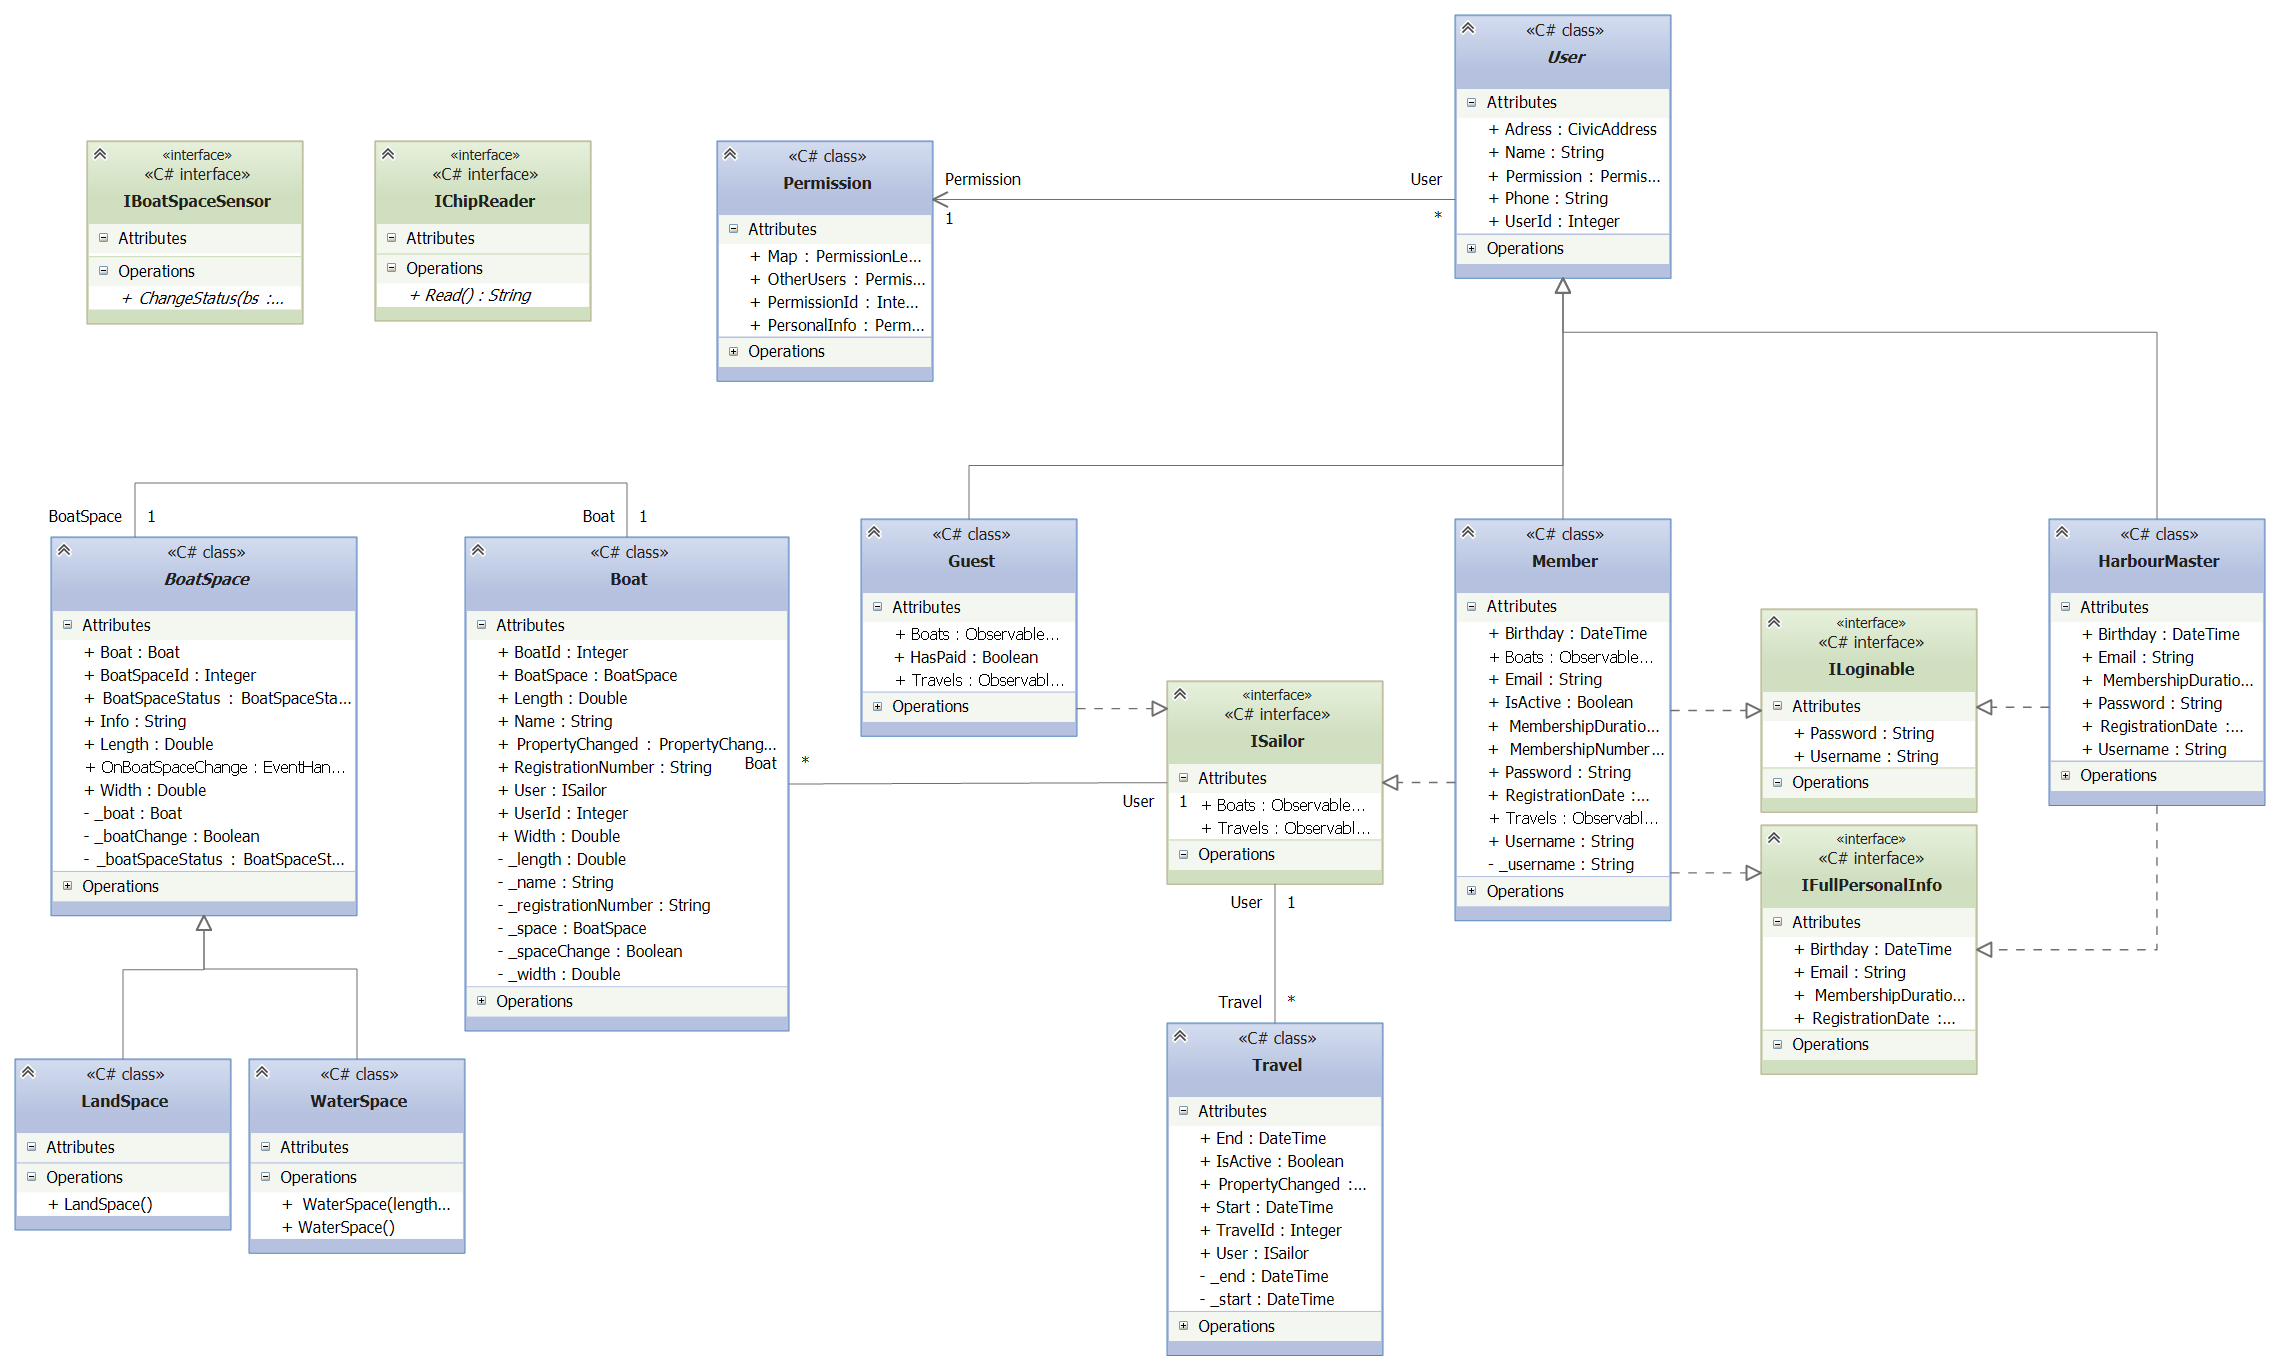
\includegraphics[width=1.2\paperwidth, angle = 270]{UML.png}
  }
 	\caption{UML-klassediagram over klasser der bruges til at modellere løsningen.} \label{fig:UML}  
 \end{figure}

\alnote{skriv om de to ensomme interfaces}

\subsection{Modellering af Brugere}
\label{sub:brugere_af_programmet}

I klassehierarkiets top ligger den abstrakte klasse \enquote{User}. En \enquote{User} er en generel bruger af systemet. Denne klasse definerer alle fællestræk de nedarvende klasser skal have. Dette inkluderer brugerrettigheder og basale informationer som telefonnummer, navn og adresse. Der findes tre forskellige interfaces, der indeholder forskellige informationer om brugere: \enquote{IFullPersonalInfo}, \enquote{ISailor}, \enquote{ILoginable}.

Subklasserne til \enquote{User} opdeler brugere som enten medlemmer af klubben, gæster eller havnefoged. Til disse tre brugertyper bruges klasserne \enquote{HarbourMaster}, \enquote{Guest} og \enquote{Member}. Denne opdeling er lavet fordi der indgår forskellige felter på tværs af disse subklasser, og de tre brugertyper er helt forskellige kategorier i programmet. 

For at differentiere subklasserne, implementeres forskellige kombinationer af interfaces. Eksempelvis må en havnefoged ikke have en båd, og derfor implementerer klassen \enquote{HarbourMaster} ikke \enquote{ISailer} interfacet. Til gengæld deler \enquote{HarbourMaster}, \enquote{IFullPersonalInfo} og \enquote{ILoginable} med \enquote{Member} klassen, da de begge har behov for at gemme mere personinformation, samt at kunne logge ind med brugernavn/medlemsnummer.
 
\subsection{Modellering af Rejser}
\label{sub:rejser}

En medlems rejse modelleres med klassen \enquote{Travel}. Den indeholder information om rejsen start- og slutdato. \enquote{Travels} bruges også til at angive hvor lang tid en gæst ligger i havnen. \enquote{Travel} implementere \enquote{IEquatable} interfacet, som gør det muligt at sammenligne med andre klasser af samme type. Klasser der implementere ISailor indeholder en liste af \enquote{Travels}.
 
\subsection{Modellering af Både}
\label{sub:bade}

Der er lavet en klasse til både, der hedder \enquote{Boat}. Denne klasse bruges til at gemme data tilhørende en båd. Der gemmes dens navn og størrelse, så man kan tjekke hvorvidt en given plads er stor nok til at rumme båden.

\subsection{Modellering af Bådpladser}
\label{sub:pladser}

Der er to klasser til repræsentation af bådpladser. Klassen \enquote{WaterSpace} modellere vandpladser og \enquote{LandSpace} modellere landplads. Begge disse klasser nedarver fra klassen \enquote{BoatSpace}, som indeholder generelle informationer om en bådplads. 

\subsection{associationer}
\label{sub:associationer}

I klassehierarkiet benyttes to typer associationer binær associationer og en-til-mange associationer. Den binære association på \cref{fig:UML} mellem både og bådpladser viser at der er en reference inderhold i båden til dens tilhørende bådplads, og vise versa. Denne association håndter at en båd tildeles en plads, får samme plads også tildelt en reference til båden. Association sikker derved også at man ikke kan tildele en plads en båd, hvis pladsen allerede inderholde en reference til en anden båd. 

En ISailor indeholder en liste til boats og en liste til Travels, mens Travels og både kun inderholder en reference til en ISailor. Dette udgør en én-til-mange association fra ISailor til boats. Denne association sikre at tilføjes et objekt til en liste inderholdt i en ISailor, tildeles objektet automatisk en reference til samme ISailor. Hvis en båd får tildelt en ISailor som sin ejer, tilføjes båden også til listen af ejerens Både. 



\section{Reflektion}
\label{sec:reflektion}

\kanote{mangler noget definition af metode}

Reflektion er en måde i C\# til at undersøge objekter i et program ved kørselstid \cite{michaelis2012essential}. Et eksempel på brugen af reflektion kan være, at programmøren ønsker at finde et felt i en klasse ved navn.

I dette projekt bruges reflektion til at gøre metoder der tilgår databasen, meget generiske, hvilket sikrer stor kodegenbrug. Som beskrevet i \cref{sec:database}, består databasen af forskellige tabeller, herunder \enquote{Users}, \enquote{Boats}, \enquote{BoatSpaces} og \enquote{Travels}. Lad os forestille os en metode der skal slette et objekt fra en specifik tabel. Metodesignaturen for en sådan metode kunne se ud som vist i \cref{lst:reflektion_remove1}.


\begin{lstlisting}[label=lst:reflektion_remove1]
public void RemoveUser(User user)
\end{lstlisting}

Problemet med denne metode er at denne metode kun virker på \enquote{User} objekter. Dette betyder at der udover denne metode også skal skrives en \enquote{RemoveBoat}, \enquote{RemoveBoatSpace} og en \enquote{RemoveTravel} metode. For at undgå dette, kan der laves en \enquote{Remove} metode, med en parameter der afgør hvilken tabel der skal slettes noget i. Metodesignaturen kunne se ud som i \cref{lst:reflektion_remove2}.


\begin{lstlisting}[label=lst:reflektion_remove2]
public void Remove<T>(T item, string table)
\end{lstlisting}

Problemet er, at metoden \enquote{Remove} skal have \enquote{hard-codet} alle de forskellige navne på alle eksisterende tabeller ind i denne metode. Hvis navnet på en tabel så ændrer sig, vil metoden ikke længere virke.

For at løse ovenstående problemer kommer reflektion ind i billedet. Metoden VerifyTable som ses i \Cref{lst:reflektion_verifytable} er et kodeeksempel fra programmet. VerifyTable bruger reflektion til at gennemsøge en klasse, her LobobContext, for at finde en egenskab af typen DbSet<T>. DbSet<T> er en databasetabel der gemmer oplysninger af typen T. Hvis den ønskede tabel bliver fundet, returneres denne. Hvis ingen tabel bliver fundet, returneres null. Først finder metoden alle egenskaber der er defineret på typen \enquote{LobobContext}. DBsetType er den egenskab der ønskes fundet. Metoden itererer nu alle egenskaber igennem, indtil en egenskab der matcher DBsetType er fundet. Hvis der er et match i foreach løkken, findes egenskab navnet, og lægges over i dbSetTarget. Det er nu muligt at dynamisk oprette en DbSet<T> ud fra typen \enquote{LobobContext}. Denne DbSet<T> returneres, og kan nu bruges i en \enquote{Remove} metode.

\begin{lstlisting}[label=lst:reflektion_verifytable, caption={Metode der tjekker om en tabel af typen T findes i databasen.}]
private DbSet<T> VerifyTable<T>(LobopContext context) where T : class
{
    Type lobobContextType = typeof(LobopContext);
    PropertyInfo[] properties = lobobContextType.GetProperties();
    Type DBsetType = typeof(DbSet<T>);
    string dbSetTarget = string.Empty;

    foreach (PropertyInfo item in properties)
    {
        if (DBsetType == item.PropertyType)
        {
            // table found
            dbSetTarget = item.ToString().Split(' ')[1];
            DbSet<T> dbSet = (DbSet<T>)lobobContextType.GetProperty(dbSetTarget).GetValue(context, null);
            return dbSet;
        }
    }
    // table of type not found
    return null;
}
\end{lstlisting}

\begin{lstlisting}[label=lst:reflektion_remove3, caption={Remove metode der kan tage en vilkårlig klasse ind, finde den rette tabel og derefter slette det parametiserede objekt}]
  public void Remove<TInput>(TInput item) where TInput : class
  {
      using (var db = new LobobContext())
      {
          DbSet<TInput> dbSet = VerifyTable<TInput>(db);
          if (dbSet == null) throw new KeyNotFoundException("table ikke fundet");
          dbSet.Remove(item);
          db.SaveChanges();
      }
  } 
\end{lstlisting}

Den færdige Remove metode der er generisk, virker nu på tværs af alle klasser, ved hjælp af reflektion. En forsimplet implementation der benytter VerifyTable af Remove meotden ses i \cref{lst:reflektion_remove3}. Hvis en Titanic båden skal fjernes fra \enquote{Boats} tabellen, kaldes koden set i \cref{lst:reflektion_remove4}. Der er nu ingen behov for at specificere i hvilken tabel titanic skal fjernes fra, da Remove selv kan regne dette ud udfra den generiske typeparameter <Boat>.

\begin{lstlisting}[label=lst:reflektion_remove4]
Remove<Boat>(titanic);
\end{lstlisting}

\section{Håndtering af Brugertilladelser} % (fold)
\label{tilladelser}

De forskellige aktører for systemet, har forskellige niveauer af tilladelser i havnen. Eksempelvis skal havnefogeden have adgang til at se alle medlemmernes rejser, i modsætning til et menigt medlem, der kun har adgang til at se sine egne rejser. For at kunne korrekt modellere de administrative ansvarsområder, er det nødvendigt at kunne skelne i mellem brugere, og deres tilladelser.

Der findes tre grader af brugertilladelse, ingen, læse eller skrive. Graden \enquote{ingen}, er den laveste grad, og betyder at den respektive bruger ikke har nogen som helst form for adgang til de pågældende datafelt. Graden \enquote{læse} gør datafeltet synligt for brugeren. Graden \enquote{skrive} giver brugeren mulighed for at redigere datafeltet. Brugertilladelser er akkumulerende, således at skrivetilladelsen implicit også er en læsetilladelse. 

Alle brugere har for ethvert datafelt én af de tre grader af brugertilladelser. Dette giver mulighed for at differentierer imellem forskellige instanser af brugermodellen, således at det ikke er nødvendigt at oprette en ny brugermodel, for enhver kombination af brugertilladelser.

Brugere tilgår systemet via et chipkort, som indeholder information der kan identificere brugeren data i systemet. Det er også muligt for medlemmer at tilgå systemet via deres medlemsnummer og et kodeord.

Når en bruger tilgår systemet, bliver programmet initialiseret, ud fra de tilladelser brugeren har. Synligheden bliver på denne måde begrænset, således at al information ikke er frit tilgængeligt, samt at brugergrænsefladen holdes så relevant som muligt.

\kanote{kodeeksempler  + forudgående tekst}

\kanote{husk mulighed for ny gæst}
\section{Moduler}
\label{sec:moduler}
\frnote{hvorfor deler vi det op i moduler?}

Moduler i dette afsnit defineres som logisk grupperede funktionaliteter og modeller i løsningen. Hvert modul skal være uafhængig af andre moduler, og kun have et enkelt ansvar, og skal udelukkende håndtere sit eget ansvar. Et login modul skal derfor ikke have ansvaret, for at oprette en ny bruger. I stedet vil et dedikeret modul, til at oprette nye brugere, være favorabelt. Hvis hvert modul kun har et enkelt ansvar, kan moduler nemt genbruges i andre sammenhænge, eller udskiftes efter behov.

Modulerne i løsningen er beskrevet ved modulets funktionalitet, brugen af andre modeller og hvordan modellen overordnet er implementeret.

Kun de hidtil implementerede moduler er beskrevet i dette afsnit. I den fulde løsning, skal flere moduler implementeres, når funktionaliteten af løsningen skal øges. De beskrevne moduler er tænkt som en grobund for efterfølgende moduler.

\sinote{Diagram over alle moduler}
\begin{figure}
  \centering
  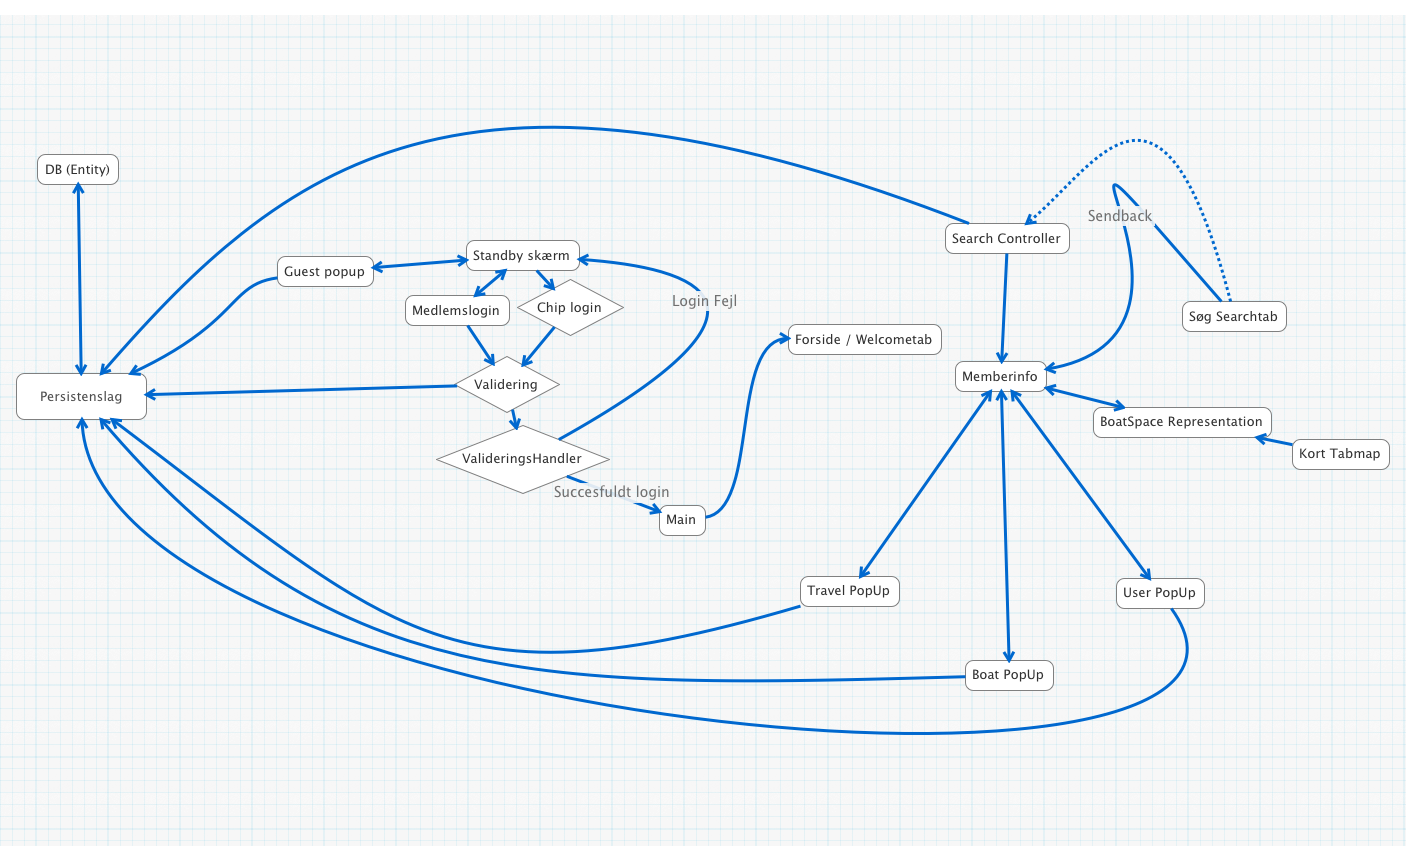
\includegraphics[width=\textwidth]{moduler_oversigt.png}
  \caption{Overordnet oversigt over moduler i løsningen og deres relationer.}
\end{figure}

\subsection{Login}
\label{sub:database}

\kanote{mangler diagrammer og kodeeksempler}

Det første modul der interageres med, er login modulet, som har til formål at validere, og videresende brugeren til programmets hovedfunktioner. Login modulet har det primære ansvar for at angive adgangsniveauer, og sikre databeskyttelse. Fra login modulet kan man vælge at oprette sig som ny gæst, eller logge ind i systemet. Hvis brugeren vælger at oprette sig som ny gæst, så vil brugeren blive sendt til et separat modul.

Login modulet består af et standby- , medlemslogin-, validerings-, samt videresendings-element.

Standby-elementet er udgangspunktet for al interaktion med programmet, og har henvisninger til hvordan brugeren anvender programmet. 

Fra standby-elementet kan brugeren vælge at gå til medlemslogin-elementet, hvor en bruger der er medlem kan logge sig ind med sit medlemsnummer, og et kodeord.

Alternativt kan brugeren indsætte et chipkort fra standby-elementet, og så sender standby-elementet brugeren direkte til validerings-elementet.

Medlemsnummeret og kodeordet bliver videresendt til validerings-elementet, som krydstjekker informationerne via databasemodulet. Validerings-elementet videresender herefter en boolsk statusmelding, samt en brugerprofil fra databasen til videresendings-elementet.

Videresendings-elementet tjekker status meldingen. Hvis meldingen er falsk, sender den brugeren tilbage til enten medlemslogin eller standby, med en passende fejlmelding. Hvis valideringen gik godt, så videresendes brugeren til Hovedmodulet.
\subsection{Styringsmodulet}
\label{sub:styringsmodul}

Styringsmodulet har til opgave at instantiere og kontrollere de moduler som udgør specifikke funktionaliteter for brugeren.

\subsubsection{Funktionalitet}
\label{ssub:hovedmodul_funktionalitet}

Når en bruger har været igennem en succesfuld validering fra loginmodulet, bliver brugeren sendt videre til styringsmodulet. Dette modul fungerer som skelettet for de omkringliggende moduler. Brugeren bevæger sig derfor hele tiden rundt indenfor dette moduls rammer, indtil brugeren ønsker at forlade programmet. Da styringsmodulet ikke selv indeholder noget information direkte til brugeren, bør den altid instantiere et default element.

\subsubsection{Implementation}
\label{ssub:hovedmodul_implementation}

\begin{figure}
  \centering
  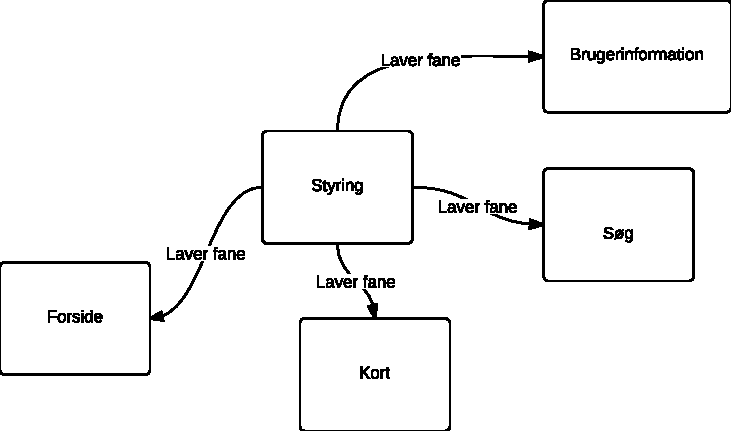
\includegraphics[width=\textwidth]{Main.pdf}
  \caption{Dette er bare noget filler tekst.}
\end{figure}


Styringsmodulet implementeres som en tabcontroller, der tilføjer andre moduler som faneblade. Default fanebladet er forsidemodulet. Dertil tilføjer styringsmodulet en kortfane, en brugerinformationsfane samt en søgningsfane. Disse faner bliver dog kun tilføjet, hvis brugeren, som er logget ind, har de nødvendige tilladelser. Når brugeren ønsker at forlade programmet, logges der ud, og brugeren sendes tilbage til loginmodulet.

\subsection{Persistenslag}
\label{sub:persistenslag}

\subsubsection{Funktionalitet}
\label{ssub:persistenslag_funktionalitet}

Persistenslag modulet har til opgave at manipulere og læse data fra en datastruktur. En datastruktur kunne f.eks. være en database eller en anden fil på harddisken. modulet tilbyder basale CRUD (create, read, update og delete) operationer, hvorfra alle tænkelige persistenslagsoperationer kan opbygges af.

Et eksempel på brugen af persistenslag modulet, kunne være login modulet. Login modulet skal verificere om et indtastet brugernavn matcher et indtastet kodeord. Til dette kan login modulet tilgå databasen igennem persistenslagets read operation, og herfra arbejde videre på den fundne data.


\subsubsection{Iplementation}
\label{ssub:persistenslag_implementation}

\frnote{Et billede med lidt tekst}

Persistenslag modulet er opbygget således at selve datastrukturen der manipuleres og læses fra, kan ændres. Herved indkapsles tilgangen til datastrukturen på en sådan måde, at et program kan gå fra at benytte en xml fil som data lager, til at benytte en database uden at ødelægge anden eksisterende kode.

Dette implementeres ved at persistenslag modulet er bevidst om en konkret implementation af tilgangen til en datastruktur. Når et andet modul ønsker at lave en læse operation på persistenslag modulet, videredelegeres denne operation til den underliggende implementation af tilgangen til en datastruktur.

\subsection{Kort}
\label{sub:kort}

\subsubsection{Funktionalitet}
\label{ssub:Funktionalitet}

Kort modullet har til opgave at give et visuelt overblik over alle bådpladser der eksisterer på en havn. Kortet præsenterer bådpladsers status i form af en beskrivende farve. F.eks. er en rød bådplads en optaget bådplads. På samme måde er en grøn bådplads fri. Kortet er interaktivt forstået på den måde, at kortets informationer er spejlet fra virkeligheden. Det vil sige at når en bådplads markeres som fri af et andet modul, skifter denne bådplads sin beskrivende farve til grøn på kortet.

Når der klikkes på en bestemt bådplads på kortet, kan følgende scenarier ske afhængigt af hvilken bruger der klikker.

\begin{description}
  \item[Bruger ligger selv ved bådpladsen] Brugeren bliver sendt hen til et modul der viser oplysninger om brugeren.
  \item[Bruger er et medlem. Der ligger en anden bruger på pladsen] Hvis brugeren har adgang til at se oplysninger om andre brugere, bliver brugeren sendt hen til et modul der viser oplysninger om brugeren.
  \item[Bruger er en gæst uden en eksisterende plads. Pladsen er ledig.] Brugeren bliver sendt til et reservationsmodul.
  \item[Bruger er en gæst med en eksisterende plads. Pladsen er ledig.] Da brugeren allerede har en plads, spørges om brugeren vil flytte til den nye plads.
\end{description}

\subsubsection{Implementation}
\label{ssub:Implementation}

En bådplads på kortet har en reference til en bådplads i databasen. Når en bådplads i databasen ændrer status, notificeres kort modullet, som nu kan ændre det visuelle status.

\subsection{Pladsregistrering}
\label{sub:plads_registrering}

\subsubsection{Funktionalitet}
\label{ssub:plads_registrering_funktionalitet}

Pladsregistreringsmodulet har til opgave at videreformidle bådpladsers tilstand til modellen. Når en ændring detekteres af modulet af et separat sensormodul, skal pladsregistreringsmodulet fungere som en adapter og ændre modellen tilsvarende. En bådplads kan have følgende tilstande:

\begin{itemize}
  \item Ledig
  \item Optaget af gæst
  \item Optaget af medlem
\end{itemize}



\subsubsection{Implementation}
\label{ssub:plads_registrering_implementation}

Modulet skal være bevidst om samtlige bådpladser, således at alle bådpladser kan få detekteret ændringer i deres tilstand. 
Modulet skal kunne håndtere flere forskellige implementationer af sensorer, således at løsningen ikke er afhængig af én type sensor, men kan lade dem skifte uden komplikationer.

<<<<<<< HEAD
\subsection{Søgemodul}
\label{sub:s_searchmodul}

Søgemodulet implementerer en sorteringsfunktion, som muliggør søgning på både og brugere.

\begin{figure}
  \centering
  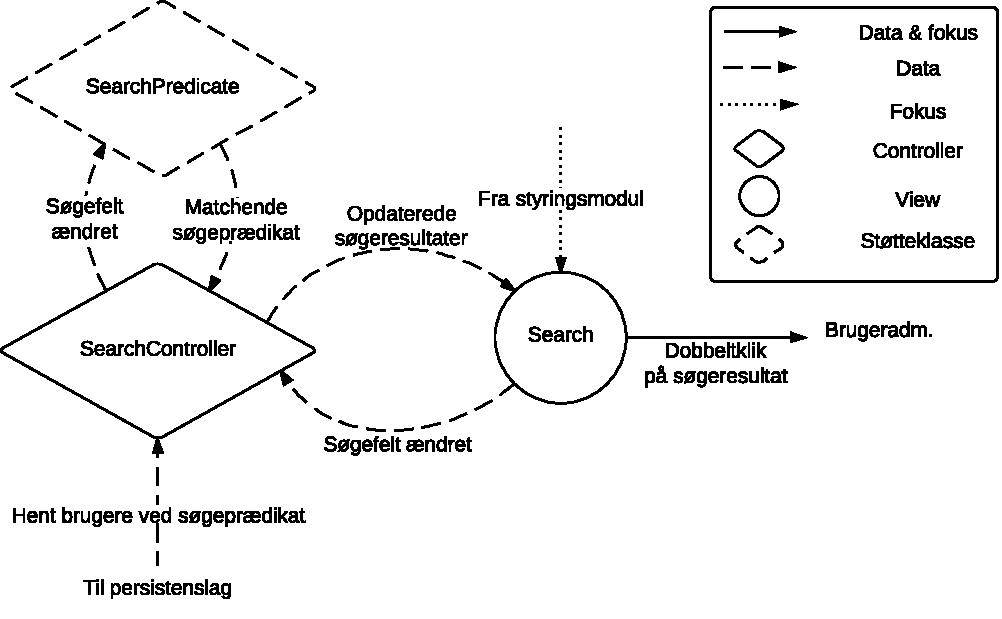
\includegraphics[width=\textwidth]{search-diagram.pdf}
  \caption{Diagram over søgemodulet}
\end{figure}
\subsubsection{Funktionalitet}
\label{sub:funktionalitet}

Søgemodulets funktion er at sortere en liste af medlemmer og gæster, ud fra brugerdefinerede kriterier. Der kan sorteres efter alle datafelter som en bruger kan have. Derudover er det muligt at sortere efter datafelter som en brugers båd eller rejser indeholder. 

\subsubsection{Implementation}
\label{sub:implementation}

Søgemodulet består af et Search-element, et SearchPredicate og en SearchController. Search-elementet tager brugerens individuelle inputs/kriterier og sender dem til SearchControlleren. SearchControlleren sender dataen til SearchPredicate som der sender et prædikat tilbage. SearchControlleren sammenligner prædikatet med persistenslaget der derefter sender \enquote{hits} tilbage til SearchControlleren. SearchControlleren sender \enquote{hits}'ne tilbage til Search-elementet der viser resultaterne i det respektive felt. Dette køre hvergang der kommer et nyt input i form af et tegn, hvilket gør at resultaterne bliver opdateret ved hvert tasteklik


% subsection implementation (end)

% subsection funktionalitet (end)

% subsection s_gemodul (end)

=======
\subsection{Medlemsinformation}
\label{sub:Medlemsinformation}

Brugerinformationsmodulet har til opgave at kommunikere mellem brugeren og databasen.

\subsubsection{Funktionalitet}
\label{ssub:Medlemsinformation_funktionalitet}

Kommunikation mellem databasen og brugeren indebærer, at vise information omkring en bruger, modtage inputs fra brugeren samt læse fra og skrive i databasen. At læse fra databasen indebærer, at den relevante information bliver hentet fra databasen, og vist på en acceptabel måde. Når der skrives til databasen menes der, at brugerens input bliver gemt i databasen. 

\subsubsection{Implementation}
\label{ssub:Medlemsinformation_implementation}

For at implementere dette består Brugerinformationsmodulet af et båd-, medlem- og rejse-delmodul. Delmodulerne har hvert deres tilsvarende ansvarsområde og er designet til at kunne læse, tilføje, redigere eller slette data fra databasen ud fra brugerens input. Læsningen af data foregår ved at et delmodul viser dets data i de respektive tekstfelter. For at redigere eller tilføje data, bliver der benyttet popup vinduer. Ved sletning af data markeres det ønskede elementer og der klikkes på fjern-knappen.
Ved at bruge popup vinduer, kan brugeren lettere kan skelne mellem at læse data og skrive data.
>>>>>>> 1eee39ea67eabb332c4cc6cbb3d7c92235169129


\chapter{Test af Implementation}



%\section{Om Systemet}
\label{sec:om_systemet}

Systemet der omtales i \cref{cha:problemformulering} tænkes at være en konsolapplikation skrevet i C\#. Programmet interagerer med en database. Denne databse gemmer alle informationer der er tilgængelige gennem programmet.

\subsection{Eksempler På Kommandoer}
\label{sub:eksempler_p_kommandoer}

Da systemet giver mulighed for at håndtere gæster, skal det være muligt at tildele en gæst til en given vandlejeplads. Nedenstående \cref{lst:add_guest} tilføjer en gæst til databasen, fortæller at han holder ved vandlejeplads 42, hedder Jens Jensen og at han har betalt indtil 1. juni 2014.

\begin{lstlisting}[language=bash, label=lst:add_guest] 
  $ program add guest --boatarea=42 --name="Jens Jensen" --until="1/6/2014" 
\end{lstlisting}


